\documentclass{article}
\usepackage[utf8]{inputenc}
\usepackage{indentfirst}
\usepackage{alltt}
\usepackage{graphicx}
\usepackage{amsmath,amsfonts,amssymb,amsthm}
\usepackage[left=2.7cm,right=2.7cm,top=2.5cm,bottom=2.5cm]{geometry}

\begin{document}
\title{Algorithmique et bioinformatique : Rapport de projet}
\author{Collin Arnaud, Galina Alicia}
\maketitle
\newpage
\tableofcontents
\newpage
\section{Introduction}
Le but de ce projet est de concevoir un programme d'assemblage de fragments ADN donnés pour fournir une séquence cohérente. Pour chaque collection de segments, une séquence cible nous est fournie pour nous assurer de l'efficacité de notre programme. Celui-ci sera développé en JAVA et abordera des notions théoriques vues en cours.

\section{Explication de la démarche}

\subsection{Structures de données}
\subsubsection{Fragment}
L'objet Fragment représente un fragment. Il contient 2 String : un contenant la chaîne de caractère associée au fragment dans le fichier FASTA et l'autre la chaîne inverse complémentaire correspondante. Il possède également une variable int id pour identifier le fragment.

\subsubsection{CollectionFragments}
L'objet CollectionFragments représente la collection de fragments encodés. Il permet de comparer facilement les fragments entre eux.
Chaque paire de segments ne doit être comparée qu'une seule fois, il est en effet inutile de comparer $s$ avec $t$ et par la suite $t$ avec $s$.

\subsubsection{Graphe}
L'objet Graphe représente le graphe de segments avec leurs scores d'alignement. Il contient 2 listes chaînées : une d'objets Node qui contient les segments et l'autre d'objets Link qui contient les scores. Il implémente aussi un algorithme de tri par tas qui classe les Link par ordre de score décroissant.

\subsubsection{Node}
L'objet Node représente un noeud du graphe, il contient différentes informations :
\begin{itemize}
\item id : un int définissant le numéro du fragment),
\item in : un booléen indiquant si nous sommes déjà rentré dans ce noeud (si il est source),
\item out : un booléen indiquant si nous sommes déjà sorti de ce noeud (si il est destination), 
\item compl : un booléen indiquant si ce segment a été choisi en complémentaire inversé. 
\end{itemize}

\subsubsection{Link} 
L'objet Link représente un lien du graphe, il contient différentes variables :
\begin{itemize}
\item sourceID : l'id du fragment source,
\item destinationID : l'id du fragment destination,
\item value : le score d'alignement de ce lien,
\item chaineSourceCompl : un booléen indiquant si le segment source est choisi en complémentaire inversé ou non,
\item chaineDestinationCompl : un booléen indiquant si le segment destination est choisi en complémentaire inversé ou non.
\end{itemize}

\subsubsection{Set}
Les objets Set représentent des ensembles de noeuds. Ces noeuds sont stockés dans une liste chaînée. Les Sets sont utilisés lors du calcul du chemin afin d'éviter les boucles.

\subsection{Algorithmes}
\subsubsection{Semi-global}
Pour définir l'algorithme semi-global, nous suivons la même implémentation que celle vue en cours. Nous devons exécuter 2 fois l'algorithme pour chaque paire de fragments. En effet, il y a 8 façons d'arranger chaque paire. Il y a 2 formes possible pour chaque fragment : normal ou complémentaire inversé. Ce qui nous donne 4 combinaisons. Pour chaque combinaison, on peut les arranger de 2 manières différentes : segment $s$ suivi de segment $t$ ou l'inverse, ce qui donne également 2 scores différents. Nous avons donc au total bien 4x2 = 8 arrangements. \\ 

Pour une combinaison, l'algorithme semi-global nous donnera ces 2 scores. A priori, il paraît nécessaire d'appliquer 4 fois semi-global à chaque paire. Cependant, il existe des combinaisons qui donnent les mêmes scores : 
\begin{enumerate}
\item la combinaison $s$ normal - $t$ normal et la combinaison $s$ complémentaire inversé - $t$ complémentaire inversé.
\item la combinaison $s$ normal - $t$ complémentaire inversé et la combinaison $s$ complémentaire inversé - $t$ normal.
\end{enumerate}
Au final, nous avons besoin d'effectuer seulement 2 fois semi-global pour calculer le score des 8 arrangements.

\subsubsection{Arrangement des liens}
Nous avons vu qu'il existe 8 arrangements différents possibles mais que certains ont le même score. Nous utilisons cet état de fait à notre avantage en stockant uniquement 4 liens au lieu de 8. En effet, pour un arrangement donné, nous savons quel autre arrangement lui correspond en terme de score. La détermination de l'arrangement à sélectionner se fera durant l'exécution de l'algorithme Greedy qui vérifiera lequel convient le mieux, si un tel arrangement existe.

\subsubsection{Tri du graphe}
Nous trions d'abord les liens du graphe par score décroissant. Pour ce faire, nous avons regroupé ces liens sous forme de tas tel que nous l'avons abordé au cours de structures de données. Cela nous permet de trouver le lien avec le score d'alignement le plus élevé en temps constant et ainsi classer rapidement les différents liens par score d'alignement décroissant.
\\

Nous avons comparé différentes structures de données possibles pour stocker les liens. Comme nous désirions avoir un tri rapide, nous avons privilégié celles ayant une complexité optimale dans le pire des cas, à savoir les structures avl et les tas(en 0(n log2 n)).
Nous avons finalement choisi d'utiliser la structure du tas (pour la complexité de la création et la simplicité de l'implémentation).

\subsubsection{Greedy}

\textbf{Sélection des liens}

\vspace{0.3mm}
Pour chaque lien stocké, nous allons vérifier si une façon d'arranger les 2 fragments est acceptable. Si oui alors on ajoute ce lien à notre chemin hamiltonien.
Lors de cette vérification, il faut être prudent car pour chaque catégorie d'arrangements, nous avons 2 scores. Si c'est l'autre façon d'arranger le lien qui doit être prise alors nous créons un nouveau lien avec les bonnes caractéristiques pour le mettre dans notre chemin. Il faut dans ce cas échanger la source et la destination pour avoir le score de même valeur dans cette disposition.\\ 

\textbf{Set}

\vspace{0.3mm}
Pour économiser du temps, nous créons les Set au fur et à mesure de la sélection des liens. Pour s'assurer de ne pas former de boucle, nous devons vérifier que la source et la destination du lien en cours n'appartiennent pas à un même Set. Si la destination et la source n'appartiennent à aucun Set, un nouveau Set est créé. Si seul l'un des noeuds du lien est présent dans un Set, l'autre  noeud est ajouté à ce Set. Si ils appartiennent à des Sets différents, alors ces 2 Sets sont fusionnés. \\ 

Comme nous utilisons des listes chaînées respectant l'ordre des noeuds pour les Sets, il suffit de faire des tests sur le premier et le dernier élément de la liste de noeuds de chaque Set sans devoir parcourir l'ensemble de cette liste lors des recherches de boucle. Notre implémentation présente aussi l'avantage de ne plus avoir qu'un seul Set contenant les noeuds du chemin dans l'ordre des chevauchements à la fin de l'algorithme. Quand le chemin hamiltonien contient le nombre de liens correspondant à une chaîne complète, alors on peut sortir de l'algorithme.

\subsubsection{Unifier} 
Nous reconstruisons le contig final à partir de 3 listes :
\begin{enumerate}
\item le Set final de Greedy : indiquant l'ordre des noeuds,
\item la liste de Node : indiquant l'orientation des noeuds,
\item la liste de Fragments : reprenant les caractères qui les composent.
\end{enumerate} 
Pour chaque noeud du Set, nous ajoutons à un String à partir du bon indice les caractères qui le compose. Cet indice est déterminé par l'indice du maximum dans la dernière colonne de la matrice obtenue par semi-global.\\

Dans notre implémentation, nous recalculons cette matrice mais nous aurions pu stocker ces indices. Nous avons pas eu l'occasion de le réaliser par manque de temps. Une fonction permettant de remonter le chemin d'alignement avait été implémentée mais n'est pas utilisée dans notre solution.


\subsection{Répartition des tâches}
Nous nous sommes répartis les tâches mais chacun a apporté des modifications au travail de l'autre. Voici la distribution des tâches :\\

\textbf{Arnaud :}
\begin{itemize}
\item Lecture et écriture du fichier FASTA
\item Objet CollectionFragments et Fragment
\item Application de l'algorithme semi-global sur l'ensemble des Fragments
\item Objet Graphe, Link et Node
\item Base du Greedy
\end{itemize}

\vspace{1.5mm}
\textbf{Alicia :}
\begin{itemize}
\item Class Algo (consacré à l'algorithme semi-global ainsi que recherche dans la matrice)
\item Création des liens et gestion des différents cas dans Greedy
\item Objet Set
\item Class Unifier
\item Rapport
\end{itemize}
\section{Points forts, points faibles et erreurs connues}
\textbf{Points forts}
\vspace{1.5mm}

Une fois le graphe créé, cela va très vite pour générer la séquence grâce au tri optimal et au nombre minimal de liens, même pour les collections les plus grandes.\\

\textbf{Points faibles}
\vspace{1.5mm}

Nous ne gérons pas le cas où des fragments seraient inclus dans un autre, ce qui entraîne sûrement une séquence plus grande.
Une idée était de supprimer totalement ces fragments et d'arrêter de calculer les alignements dès qu'une inclusion était détectée. Il aurait cependant fallu remonter le chemin de la matrice semi-global à chaque fois, ce qui aurait été fort couteux en temps, surtout pour les plus grosses collections. \\

\textbf{Erreurs}
\vspace{1.5mm}

A priori, nous n'avons pas remarqué d'erreurs.

\section{Interprétation des résultats obtenus}
Pour toutes les collections, le dotmacher de la séquence normale était le meilleur.
Souvent, le dotmatcher de la séquence inversée complémentaire ne présentait aucune droite. Nous ne présenterons donc que  résultats pour les séquences normales.\\

Pour la collection 1 simplifiée, le dotmatcher est bon : notre séquence recouvre toute la séquence cible et elle est à peu près de même taille.
\begin{center}
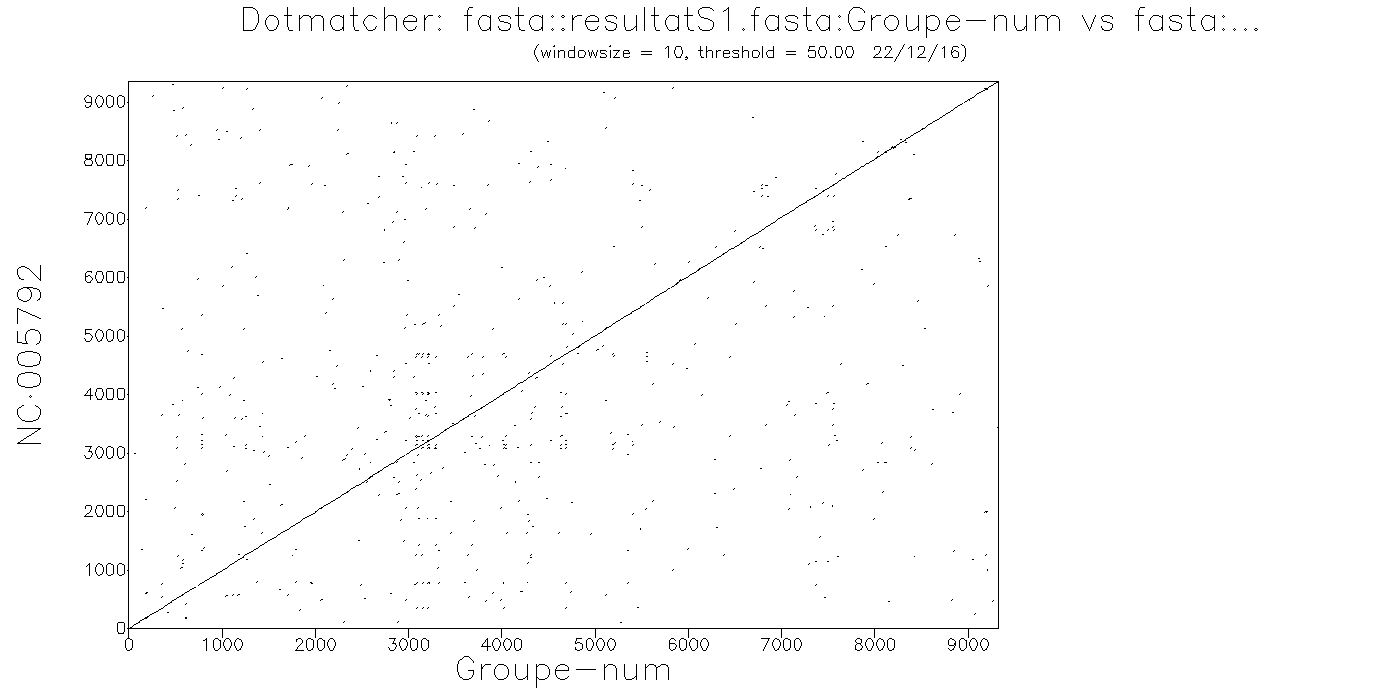
\includegraphics[scale=0.4]{dotmatcher1S.png}
\end{center}

Pour la collection 1, 4 et 5, nous constatons que les séquences cibles sont couvertes mais nos séquences sont trop grandes : environ le double à chaque fois.

\begin{center}
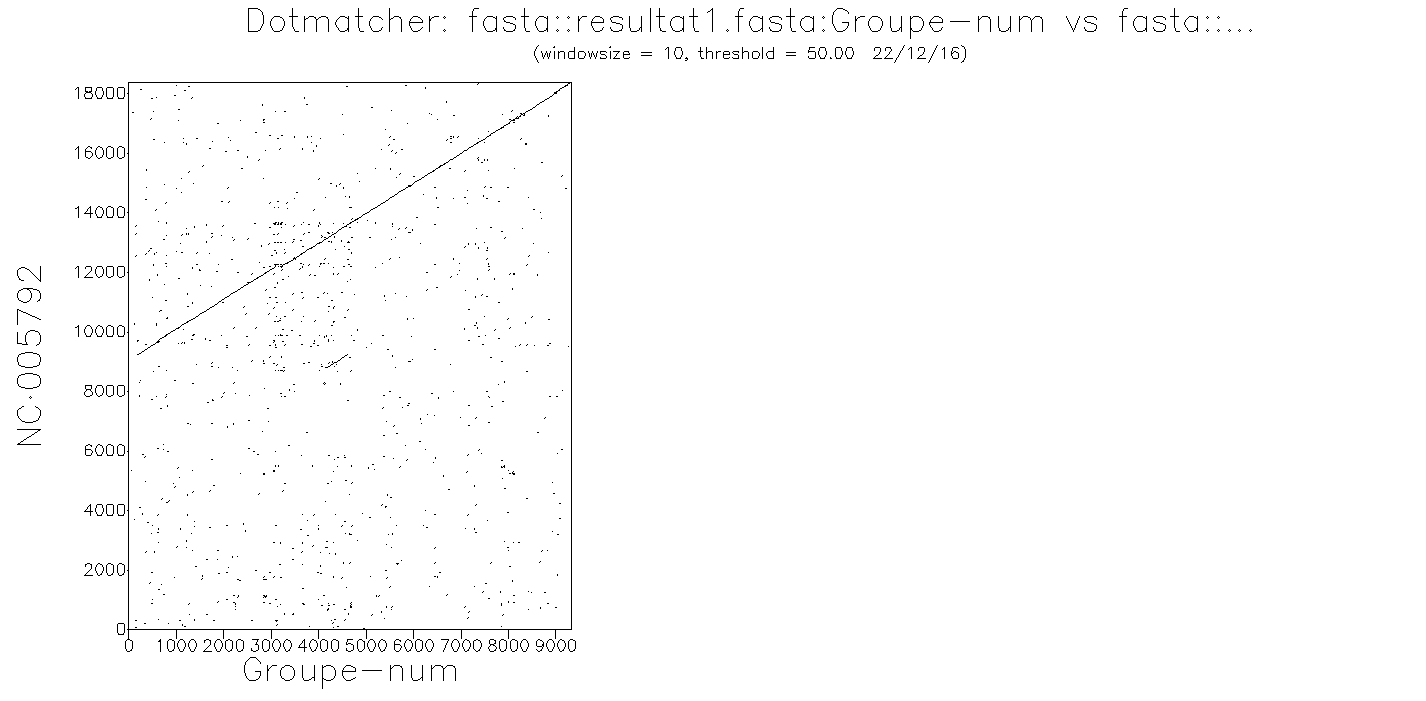
\includegraphics[scale=0.5]{dotmatcher1.png}
\end{center}

\begin{center}
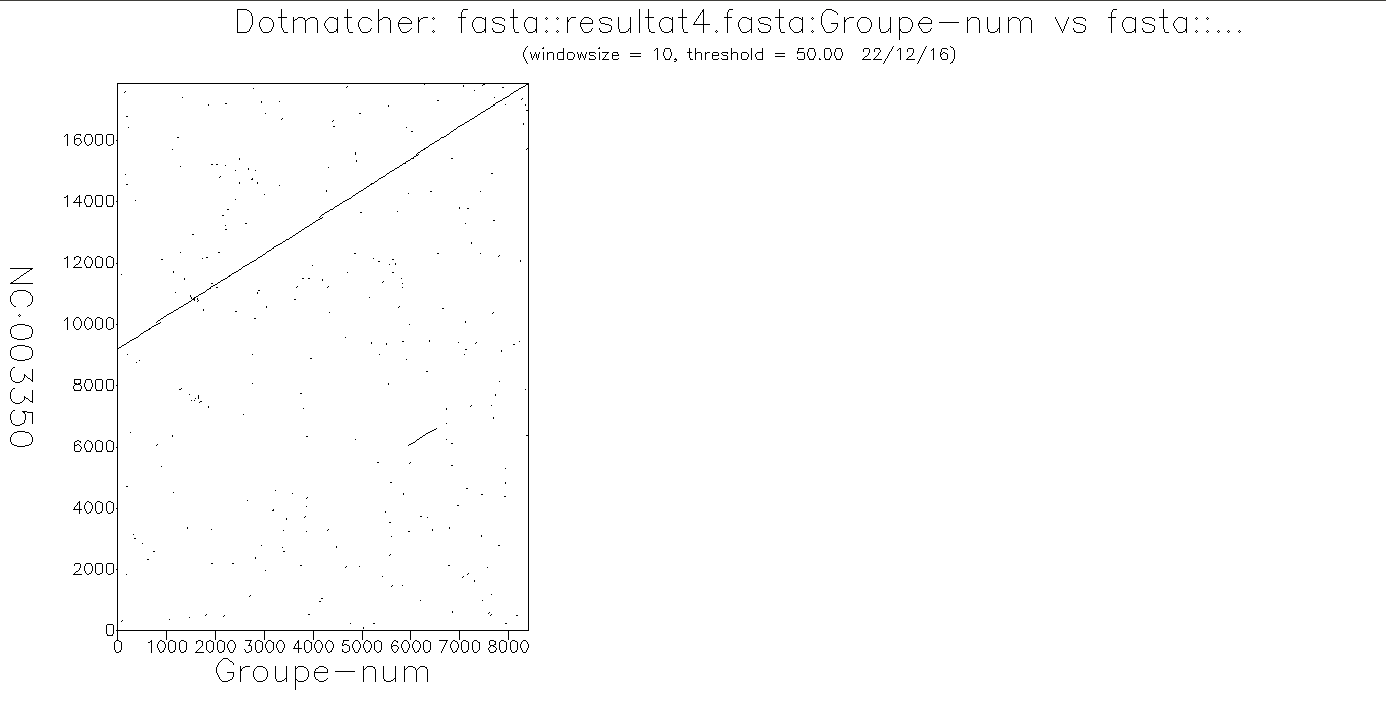
\includegraphics[scale=0.5]{dotmatcher4.png}
\end{center}

\begin{center}
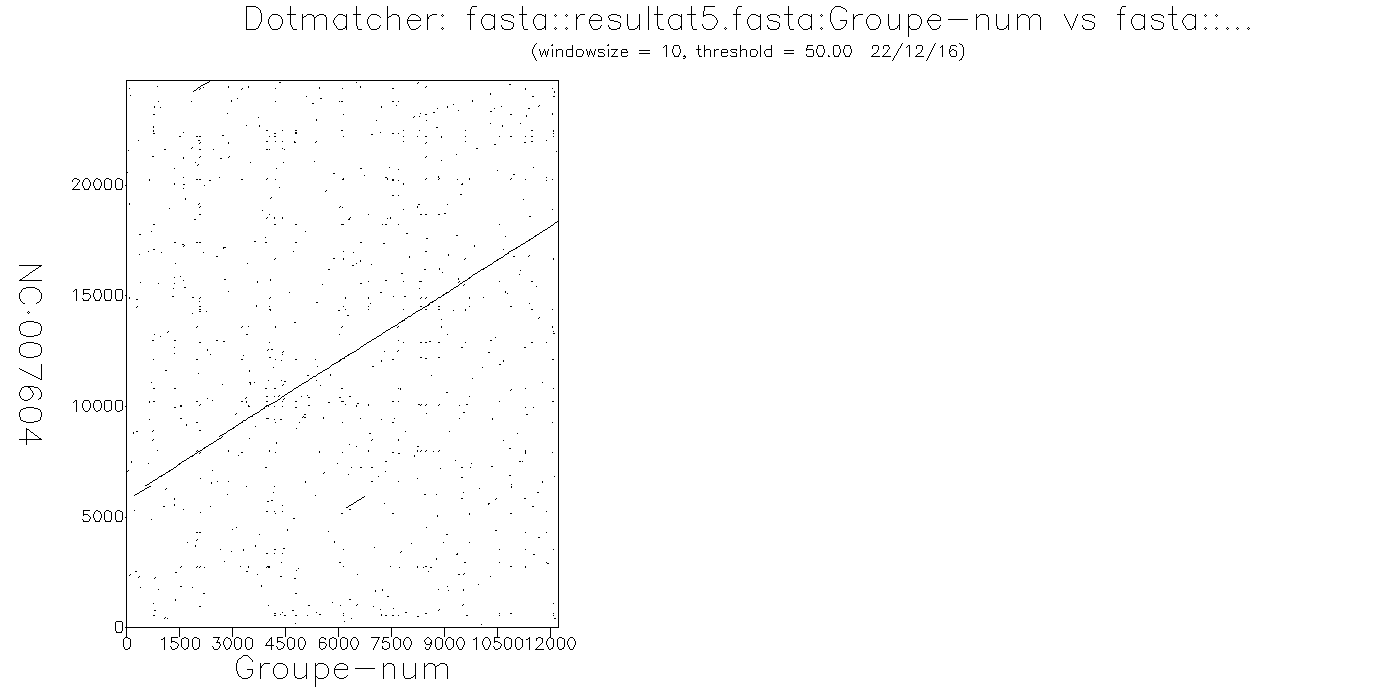
\includegraphics[scale=0.5]{dotmatcher5.png}
\end{center}

Le dotmatcher de la collection 2 est beaucoup plus flou. On observe encore une fois que toute la séquence est recouverte bien qu'elle soit plus éparpillée. Sa taille est aussi trop grande.
\begin{center}
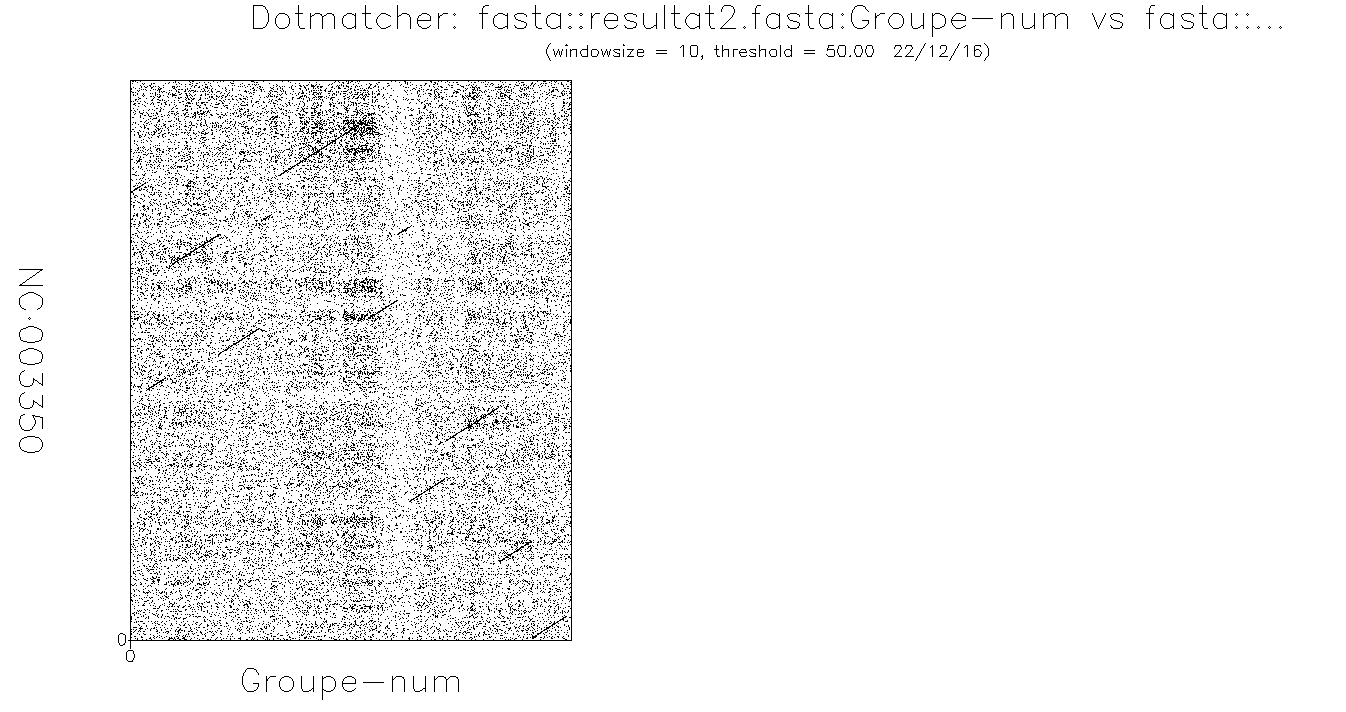
\includegraphics[scale=0.5]{dotmatcher2.png}
\end{center}

\newpage
\section{Conclusion}
L'assemblage de fragments est un problème très complexe. Il faut parvenir gérer une très grande quantité de données. De plus l'approximation de type Greedy exclut certaines possibilités d'assemblage : nous sommes obligés d'assembler les fragments en escalier. Or, en réalité, ils se chevauchent probablement tous de manière aléatoire.  \\
\begin{center}
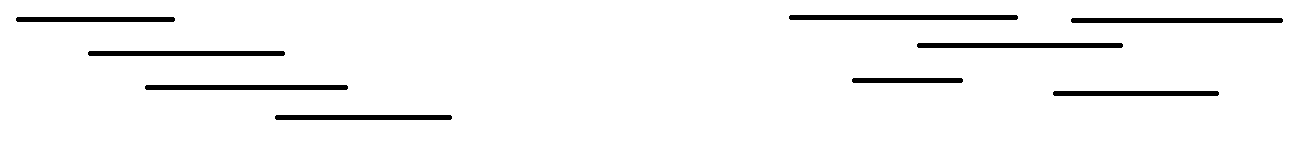
\includegraphics[scale=0.5]{alignement1.png}
\end{center}

Nous pensons que cela peut avoir un impact sur la longueur des séquences obtenues. \\

Nous avons eu des difficultés au niveau de la bonne compréhension des alignements afin d'effectuer le minimum de Semi-global et de stocker le minimum de liens. Comme nous ne stockons seulement que la moitié des liens possibles, il a fallu déterminer quels alignements avaient les mêmes coûts et les vérifier dans Greedy.
\end{document}
